\section{Experiments}\label{sec:experiments}
To demonstrate our {\em GeoTracking} and {\em GeoRouting} extension
blocks and our {\sc breadcrumb} router, we used our implementations of
them in the IBR-DTN core and with the Java API and performed
end-to-end experiments on the VirtualMeshTest (VMT) channel-emulated
testbed~\cite{hahn10:using, kim11:reality}.  VMT uses Linux-based real
wireless nodes with commodity wireless hardware to emulate mobile
environments.  The wireless testbed is effectively an analog channel
emulator based on an array of programmable attenuators.  Given a
desired physical arrangement of nodes, the system computes the
expected path loss between nodes and programs the attenuators
accordingly.  VMT updates the attenuations every second to emulate a
mobile wireless environment.

For each of our experiments, we define one node to be a {\em
  sender} and another to be a {\em responder}. Using the Java IBR-DTN
bridge API, we used our application to create application-level
bundles that we sent through our router. The {\em sender} initially
creates a probe bundle, to which it attaches a {\em GeoTracking}
extension block. The {\em sender} then sends this bundle to the {\em
  responder} using his EID as the target of routing. When the {\em
  responder} receives this bundle at the application level, it creates
a bundle with a {\em GeoRouting} tracking block that specifies as
waypoints a subset of the locations visited by probe. The geo-routed
bundle is sent back along the waypoints.

%{\bf The Ladder.} The first scenario contains thirteen nodes. Eight of
%the nodes form two evenly spaces parallel lines; these form the sides
%of the ladder. One node sits, stationary, at the bottom of the ladder;
%another node sits, stationary, at the top of the ladder. Three nodes
%repeatedly climb from the bottom of the ladder to the top and back
%down. {\color{red} The sender is at the top of the ladder and the
 % responder at the bottom; Figure~\ref{fig:ladder1} shows the
  %trajectory of the responder's geo-routed bundle, with the target
  %location waypoints from the {\em GeoRouting} extension block
  %highlighted.}
%\begin{figure}
%\begin{center}
%\begin{tikzpicture}
%\begin{axis}[legend pos=south east]
%\addplot+[only marks,color=black,mark=*,mark size=0.2pt] 
%	table[x=x,y=y] {../data/ladder/pgy.txt};
%\addplot[only marks,color=red,mark=x] 
%	table[x=x,y=y] {../data/ladder/pgy_2.txt};
%\legend{Bundle Trajectory}
%\end{axis}
%\end{tikzpicture}
%\end{center}
%\vspace{-.75cm}
%\caption{Ladder Experiment 1}\label{fig:ladder1}
%\vspace{-.5cm}
%\end{figure}

{\bf Crop Circles.} In our first set of experiments, we created grids
of nodes that move continuously in circles in either a clockwise or
counter clockwise pattern. These {\em crop circles} consist of six
nodes arranged as in Figure~\ref{fig:cropcircle1}; the sender is the
node in the lower left; the responder is the node in the upper right.
Figure~\ref{fig:cropCirclesExperiment} shows the results of a single
execution on the crop circles network;
Figure~\ref{fig:cropCirclesExperiment}(a) shows the trajectory of the
probe bundle sent from the sender to the responder, while
Figure~\ref{fig:cropCirclesExperiment}(b) shows the trajectory
followed by the return (geo-routed) bundle. The small circles indicate
the waypoints specified in the {\em GeoRouting} block of the
responder's bundle (which were computed automatically by our
application layer from the probe's {\em GeoTracking} block).
\begin{figure}[!h]
\vspace{-.2cm}
\begin{center}
%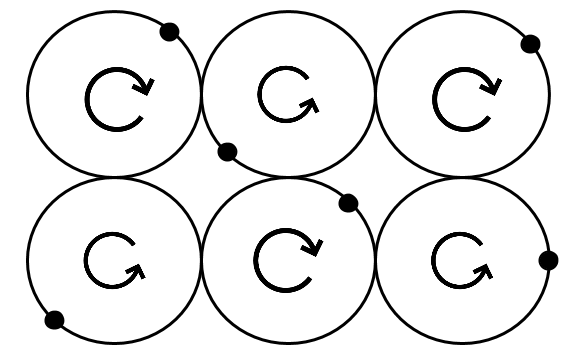
\includegraphics[width=\columnwidth+.5]{figures/cropcircle1.png}
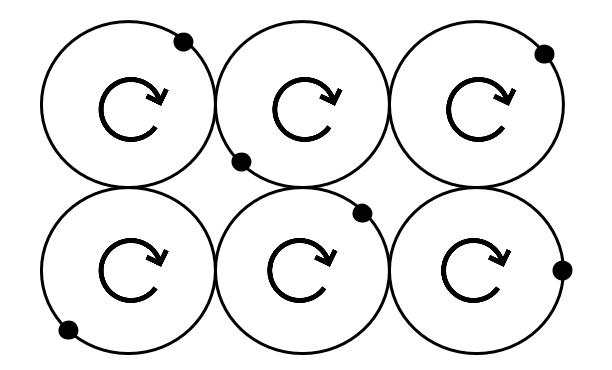
\includegraphics[width=.65\columnwidth]{figures/cropcircles2.png}
\end{center}
\vspace{-.75cm}
\caption{Crop circles mobility scenario}\label{fig:cropcircle1}
\vspace{-.25cm}
\end{figure}

The track of the sender's probe bundle stops as soon as the responder
(the node in the upper right corner) receives the bundle. When the
responder generates its {\em GeoRouting} block for the return bundle,
it inserts its location as the first waypoint. The track of the
responder's bundle (Figure~\ref{fig:cropCirclesExperiment}(b)) hits
all of the waypoints specified in the {\em GeoRouting} bundle. In the
figure, the final waypoint does not appear to quite be reached. This
is because our experiments deserialize and log the tracking blocks
only when a bundle arrives at a node; once the node in the top left
corner hands the bundle to the node in the lower left corner, the
latter node continues to move along the path shown in
Figure~\ref{fig:cropcircle1}, eventually crossing that final waypoint.
\begin{figure}[!h]
\begin{center}
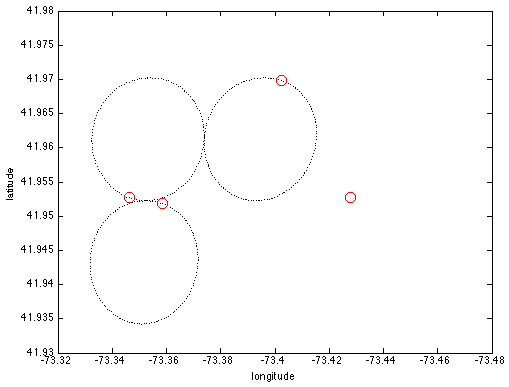
\includegraphics[width=.8\columnwidth]{figures/CropCirclesExperiment2.png}\\
(a)\\
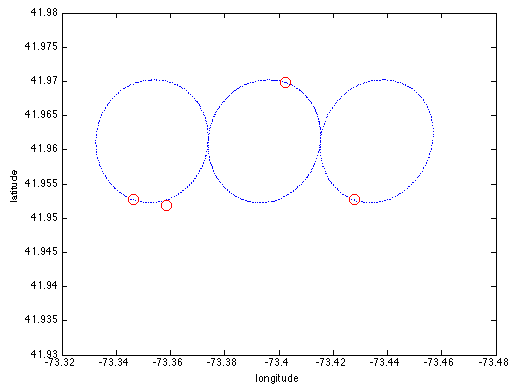
\includegraphics[width=.8\columnwidth]{figures/CropCirclesExperiment.png}\\
(b)\\
\end{center}
\vspace{-.5cm}
\caption{Crop circles tracking and trajectories. (a) The tracked
  trajectory of the probe bundle. (b) The tracked trajectory of the
  geo-routed bundle.}
\label{fig:cropCirclesExperiment}
\vspace{-.25cm}
\end{figure}


{\bf The Maze.} Our final experiments mirror the motivating scenario
of the prisoner in the maze. The maze consists of a series of
connected hallways, each patrolled by a single guard who moves back
and forth along hallway. Our maze is shown in
Figure~\ref{fig:maze}. The sender (i.e., the prisoner) is the node in
the lower left corner, while the responder (i.e., the rescuer) is the
node in the lower right corner.
\begin{figure}
\begin{center}
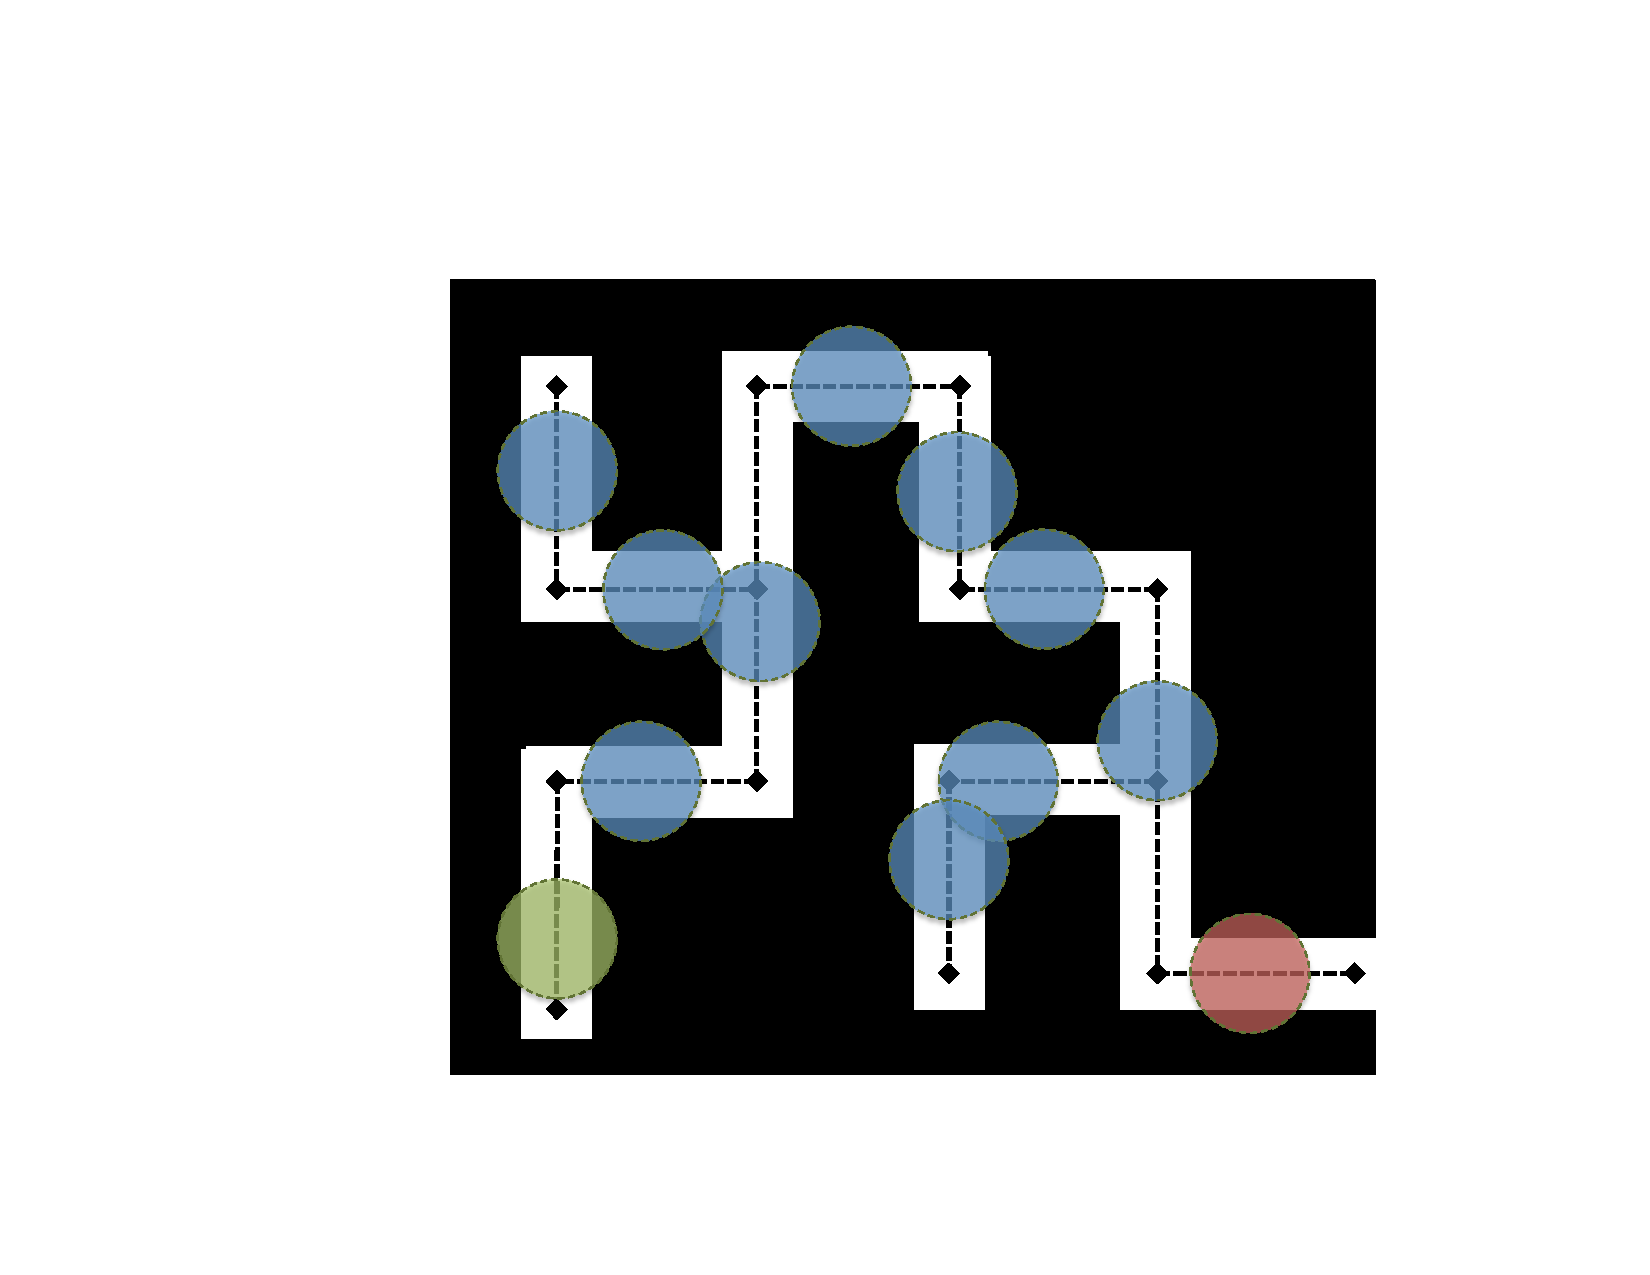
\includegraphics[width=.7\columnwidth]{figures/newMaze.pdf}
\end{center}
\vspace{-.75cm}
\caption{Maze mobility scenario}
\label{fig:maze}
\vspace{-.25cm}
\end{figure}

Figure~\ref{fig:mazeExperiment} shows the results of a single
execution on the maze in Figure~\ref{fig:maze}. The figure shows only
the trajectory of the rescuer's bundle that is geo-routed back to the
prisoner based on the tracked trajectory of the prisoner's probe
bundle. While copies of the prisoner's probe bundle do wander down the
maze's dead-end paths, the reply from the rescuer reflects only the
successful path through the maze. In Figure~\ref{fig:mazeExperiment},
The responder's bundle successfully reaches all of the {\em
  GeoRouting} block's required waypoints without following any
detours; the last waypoint is reached eventually, when the prisoner
moves back along his corridor.
\begin{figure}
\begin{center}
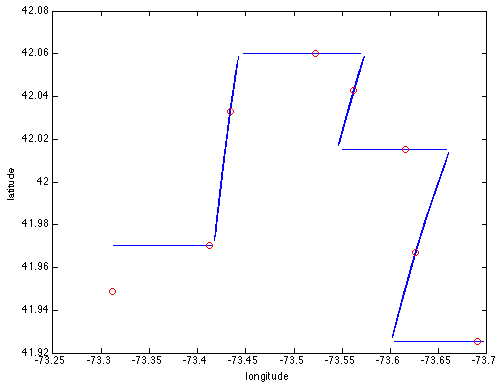
\includegraphics[width=.8\columnwidth]{figures/MazeExperiment.png}
\end{center}
\vspace{-.75cm}
\caption{Maze routing trajectory}
\label{fig:mazeExperiment}
\vspace{-.5cm}
\end{figure}
